\chapter{Speichersysteme}

Speichersysteme sind eine entscheidende Komponente der IT Infrastruktur eines Unternehmens. In der heutigen Zeit kann man von Speichersystemen kaum absehen, da Big Data immer an Wichtigkeit gewinnt. Sie bieten eine Möglichkeit, große Mengen an Daten zu speichern und zu verwalten, um den Zugriff und die Nutzung zu erleichtern. Es gibt eine Vielzahl an Speichersystemen, die für verschiedene Zwecke konzipiert sind. Durch die große Auswahl in der IT und die stetig anwachsende Innovation stellt sich die Frage, welche Speichersysteme sich für bestimmte Zwecke (Use Cases) eignen. Die Wahl des richtigen Speichersystems hängt von den Anforderungen des Unternehmens ab, wie zum Beispiel der Art der zu speichernden Daten, dem benötigten Zugriff und die Skalierbarkeit. Eine gründliche Analyse der Anforderungen und Kosten ist entscheidend, um die beste Lösung zu finden, die den Bedürfnissen des Unternehmens entspricht.\\
\\ 
Im nachfolgenden Kapitel werden die unterschiedlichen Typen von Speichersystemen vorgestellt, wobei der Fokus auf den drei Speicherarten File-, Object- und Block Storage liegt. Im Anschluss daran erfolgt ein Vergleich von zwei Cloud-Providern in Bezug auf sicherer Speicherung, Hochverfügbarkeit, Performance, Kosten, API-Anbindung sowie der Dateibereitstellung. Auf Basis dieser Kriterien wird eine Entscheidung darüber getroffen, welcher Provider den Bedürfnissen von "Leoticket" entspricht. Hierbei fließen die Kosten- und Performance-Analysen mit in die Entscheidung ein.

\section{Arten von Speichersystemen}

Im folgenden Abschnitt werden die verschiedenen Arten von Speichersystemen vorgestellt, die für die Speicherung von digitalen Daten verwendet werden. Hierbei werden die drei gängigsten Speicherarten File-, Object-, und Blob Storage behandelt.\\
 
Die heutige IT-Landschaft bietet eine Vielzahl von Speichersystemen, die je nach Bedarf und Anforderungen ausgewählt werden können. Neben den traditionellen Speichermedien wie Festplatten und Bandlaufwerken gibt es heute auch verschiedene Arten von Speichersystemen, die in der Cloud oder als lokale Lösungen bereitgestellt werden können. Dazu gehören unter anderem File Storage, Object Storage und Blob Storage.\\

Jeder dieser Speicherarten hat ihre spezifischen Vor- und Nachteile und ist für bestimmte Anwendungsfälle besser geeignet als andere. 

\newpage
 
\subsection{File Storage}

File Storage, auch dateiebenen- oder dateibasierter Storage genannt \cite{redHat-storage}, ist eine Speicherlösung bei der Dateien auf einem Dateisystem gespeichert werden. 

\begin{quote}
	Dieses System wird auch als hierarchischer Storage bezeichnet und gilt als das älteste und am weitesten verbreitete Datenspeichersystem für Direct und Network-Attached Storage. Dateisysteme organisieren Daten in hierarchischen Ordnern und Unterverzeichnissen, ähnlich wie in einem Dateiordner auf einem Computer. Dateien werden in der Regel auf einem Server oder einer Festplatte gespeichert und können von mehreren Benutzern gleichzeitig gelesen und geschrieben werden. Hierbei werden die Informationen in einzelnen Verzeichnisse abgelegt und können über den entsprechenden Pfad aufgerufen werden. Um dies zu ermöglichen, werden begrenzte Mengen an Metadaten genutzt, die dem System den genauen Standort der Dateien mitteilen, vgl. \citeauthor{redHat-storage}.
\end{quote}

In der folgenden Abbildung wird die hierarchische Struktur des Dateispeichers visualisiert.\\

\begin{figure}[h]
\centering
	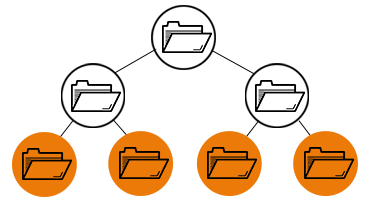
\includegraphics{Pictures/FileStorageHierarchy.png}
	\caption{File Storage: Aufbau des Hierarchiesystems, \citeauthor{redHat-storage}}
\end{figure}

File Storage wird häufig in Unternehmen und Organisationen eingesetzt, um gemeinsame Dateiserver bereitzustellen oder Daten in Cloud-Speicherdiensten wie Dropbox oder Google Drive zu speichern.
Auch wenn es von Betriebssystemen und Anwendungen gut unterstützt wird, kann die Performance und Skalierbarkeit von File Storage bei sehr großen Dateisystemen beeinträchtigt werden, was insbesondere bei stark frequentierten Anwendungen oder bei der Verarbeitung großer Datenmengen zum Problem werden kann. 

\begin{quote}
	Mit zunehmenden Datenvolumen erfordert das Skalieren von Dateispeichern das Hinzufügen neuer Hardwaregeräte oder den Austausch vorhandener Geräte durch solche mit höherer Kapazität. Dies kann im Laufe der Zeit teuer werden. \glqq As data volumes expand, scaling file storage requires [...]\grqq, (\cite{nx-fileScala}, Übersetzung des Autors)
\end{quote}

Laut Wahlmann (\citeyear{nx-fileScala}, Übersetzung des Autors) wird die Datenspeicherung bei zu vielen Daten nicht nur teuer, sondern auch unhandlich und zeitaufwändig. Der schnelle und einfache Zugriff auf jede einzelne Datei wird schwierig, wenn man zig Millionen von Dateien in Tausenden von Verzeichnissen auf Hunderten von Speichergrößen speichert. 

\subsection{Block Storage}

Block Storage, auch genannt als Block-level Storage speichert Dateien auf SAN(Storage Area Networks) basierten Netzwerken oder auf Cloud-basierten Speicherumgebungen. Das System teilt Daten in Blöcke auf und speichert die separaten Teile jeweils mit einer eindeutigen Kennung, vgl. \cite{ibm-topics}.\\

Daten werden in Blöcken auf dem Datenträger gespeichert, die unabhängig voneinander adressiert werden können. Jeder Block ist eine feste Größe, typischerweise im Bereich von einigen Kilobytes bis hin zu einigen Megabytes. Diese Blöcke können im System an jeder Stelle gespeichert werden.

\begin{quote}
	Wenn auf Block Storage gespeicherte Daten abgerufen werden, verwendet das Server-Betriebssystem die eindeutige Adresse, um die Blöcke wieder zusammenzufügen und so die Datei zu erstellen. Der Vorteil besteht darin, dass das System nicht durch Verzeichnisse und Dateihierarchien navigieren muss, um auf die Datenblöcke zuzugreifen. Dadurch werden Effizienzen erzielt, da der Abruf von Daten schneller erfolgen kann, vgl. \cite{ibm-storage}.
\end{quote}

Typische Anwendungsbereiche des Block Storage sind Datenbanken, Virtualisierungsumgebungen und Anwendungen für Big Data-Analysen. Speicherung von strukturierten Daten wie Datenbanken, Virtuelle Maschinen und Betriebssysteme eignen sich besonders bei der Verwendung von Block Storage. Diese Art von Daten erfordert schnellen und direkten Zugriff auf bestimmte Bereiche des Speichers und muss häufig in Echtzeit ausgeführt werden. Block Storage eignet sich daher am besten für Anwendungen mit hohen Anforderungen an die Leistung und niedriger Latenzzeit.

\newpage

\subsection{Object Storage}

Object Storage hat sich als Speichertechnologie in den letzten Jahren immer stärker etabliert und wird von vielen Unternehmen als Alternative zu traditionellen Speicherlösungen wie Block- oder File Storage angesehen. Die ersten Object Storage Systeme wurden bereits in den 1990er Jahren entwickelt, aber erst mit dem Aufkommen von Big Data, IoT und der Cloud-Nutzung 
 hat es einen breiteren Einsatz gefunden. Heute bieten viele Cloud Provider wie Amazon Web Services (AWS) und Google Cloud Platform (GCP) Object Storage als einen ihrer Haupt-Cloud-Services an.\\
 
\begin{quote}
	Object Storage ist für den Umgang mit großen Datenvolumen und unstrukturierten Daten entwickelt wurden. Sie speichert Daten als eigenständige Objekte, die aus Daten und Metadaten bestehen und einen eindeutigen Identifier (UID) haben (\glqq Object storage (aka object-based storage) is a type of data storage used to [...]\grqq, \cite{dataCore-OS}, Übersetzung des Autors).
\end{quote}

Im Gegensatz zu hierarchischen Systemen wie beim File Storage ist das Speichersystem flach strukturiert. Durch die einfache API Anbindung kann es mit vorhandenen Anwendungen integriert werden. Nutzer können detaillierte Informationen wie beispielsweise Erstellerangaben, Schlüsselwörter sowie Sicherheit-und Datenschutzrichtlinien hinterlegen. Diese Daten bezeichnet man als Metadaten.\\

Laut \citeauthor{nx-fileScala}, 2022 ist Skalierbarkeit der Hauptvorteil, da bei der Speicherung von Petabyte und Exabyte alle Objekte in einem Namespace abgelegt werden. Selbst wenn dieser Namespace auf Hunderte von Hardwaregeräten und Standorten verteilt ist, können alle Objekte schnell abgerufen werden. Andere Vorteile von Objekt Storage beinhalten die Datenintegritätsprüfung, im Englischen bekannt als \glqq erasure coding\grqq und die Datenanalyse.\\

Auch Object Storage hat seine Nachteile. Laut \citeauthor{redHat-storage} muss das Objekt nach der Speicherung bei Veränderung komplett neu überschrieben werden. Sie sind für traditionelle Datenbanken nicht geeignet, da das Schreiben von Objekten Zeit beansprucht und man sich mit der API auseinandersetzen muss, vgl. \citeauthor{redHat-storage}.\\

Insgesamt bietet Object Storage eine skalierbare und flexible Methode zur Speicherung von unstrukturierten Daten. Organisationen sollten jedoch die Vor- und Nachteile von Object Storage im Kontext ihrer spezifischen Anwendungsfälle abwägen, um eine fundierte Entscheidung über die beste Speichermethode zu treffen.\\

%TODO Object Storage Entscheidung

Da leoticket Daten wie Rechnungen und Tickets als Dateien speichern und abrufen abruft, ist Object Storage die richtige Speicherart. 

Für leoticket ist die Object Storage Variante die am Besten geeignetste Speicherlösung, da ... %TODO Satz weiterschreiben


\section{Aktuelle Speichertechnologien im Markt}

Die beiden größten Cloud-Speicheranbieter, Amazon Web Services (AWS) und Google Cloud Platform (GCP), bieten eine Vielzahl von Speicherlösungen an, die auf die Bedürfnisse von Unternehmen zugeschnitten sind.\\ 

In diesem Kapitel werden die aktuellen Speichertechnologien auf dem Markt untersucht, wobei der Fokus auf den Angeboten von AWS und GCP liegt. Um eine Vergleichsgrundlage zwischen AWS und GCP zu schaffen, werden die verschiedenen Aspekte wie sichere Speicherung, Hochverfügbarkeit, Leistung, Kosten, API Anbindung und die Bereitstellung der Dateien betrachtet. Dieses Vorgehen dient dazu, zu ermitteln, welche Speicherart sich am besten für welche Anforderungen eignet. Als Kontrast dazu wird das Open-Source-Objektspeichersystem MinIO betrachtet.\\

AWS bietet eine Reihe von Speicheroptionen an, darunter Amazon S3 (Simple Storage Service). Amazon S3 ist ein Object Storage-Service, der für die Speicherung und den schnellen Abruf von unstrukturierten Daten wie Videos, Fotos und Dokumenten ausgelegt ist.

Google Cloud Platform bietet ebenfalls eine Vielzahl von Speicherlösungen an, darunter Google Cloud Storage. Google Cloud Storage ist ein Object Storage-Service, der für die Speicherung von unstrukturierten Daten wie Bildern, Videos und Dokumenten ausgelegt ist.\\
 
Insgesamt bieten AWS und Google Cloud Platform eine Vielzahl von Speicherlösungen an, die auf die Bedürfnisse von Unternehmen zugeschnitten sind. Organisationen sollten jedoch die Vor- und Nachteile jeder Speicherlösung abwägen, um die beste Lösung für ihre spezifischen Anforderungen zu finden.

\newpage

\subsection{Eigenschaften}

Im vorliegenden Abschnitt werden Amazon S3 und Google Cloud Storage in Bezug auf verschiedene Kriterien untersucht. Dabei werden zunächst die Eigenschaften von AWS S3 erläutert, gefolgt von einer Betrachtung von GC Storage. Ziel ist es, die Unterschiede zwischen den beiden Anbietern hervorzuheben und eine Entscheidungshilfe zu bieten, welche Plattform für die Anforderungen von \glqq leoticket\grqq am besten geeignet ist. Die Auswahl der Kriterien erfolgt in Anlehnung an die spezifischen Anforderungen von \glqq leoticket\grqq.

%TODO Aws und GCP Definition?

\subsubsection{Sichere Speicherung}

\textbf{Amazon S3}\\

Viele Anbieter von Object Storage-Lösungen bieten integrierte Verschlüsselungsmöglichkeiten an, um sicherzustellen, dass Daten sowohl in Ruhe als auch in Bewegung geschützt sind. Dabei können unterschiedliche Verschlüsselungsmethoden zum Einsatz kommen. In Bezug auf die sichere Speicherung bieten sowohl AWS als auch GCP verschiedene Optionen für die Verschlüsselung von Daten.Die Sicherheit der gespeicherten Daten ist von entscheidender Bedeutung, um die Integrität und Vertraulichkeit der Daten zu gewährleisten. In diesem Unterabschnitt werden die verschiedenen Sicherheitsfunktionen von Amazon S3 untersucht.\\

IAM (Identity and Access Management) ist ein wichtiger Bestandteil von AWS und ermöglicht es Benutzern, Gruppen und Rollen zu erstellen, um den Zugriff auf S3 zu verwalten. Benutzer können individuelle Berechtigungen zugewiesen werden, während Gruppen und Rollen mehrere Benutzer mit denselben Berechtigungen zusammenfassen können. Auf S3-Buckets und Objekte kann man eine granuläre Zugriffssteuerung anwenden. Benutzer, Gruppen oder Rollen können so berechtigt werden, den Zugriff auf bestimmte Buckets und Objekte zu beschränken oder zu erlauben. "Beim Erteilen von Berechtigungen in Amazon S3 entscheiden Sie [...]."\cite{aws-iam-s3}\\

Eine weitere wichtige Sicherheitsfunktion von Amazon S3 ist die Datenverschlüsselung. S3 bietet eine Vielzahl von Verschlüsselungsoptionen für die serverseitige und clientseitige Verschlüsselung. Da für leoticket die clientseitige Verschlüsselung nicht in Frage kommt, liegt der Fokus auf der serverseitigen Verschlüsselung. Es gibt drei Methoden, darunter die serverseitige Verschlüsselung mit Amazon S3-verwalteten Schlüsseln (SSE-S3), mit KMS-verwalteten Schlüsseln (SSE-KMS) und die SSE-C. Diese Optionen ermöglichen es Benutzern, die Verschlüsselung auf ihre spezifischen Anforderungen abzustimmen und so die Sicherheit der Daten zu gewährleisten.

Laut \citeauthor{aws-iam-s3} nutzen Buckets standardmäßig die SSE-S3 Methode. Für die Verschlüsselung wird die 256-bit Advanced Encryption Standard (AES-256) verwendet. Seit dem 5. Januar 2023 sind alle neu erstellen Buckets auf SSE-S3 ausgelegt. Alle neuen Objekte sind beim Hochladen automatisch verschlüsselt, ohne weitere Zusatzkosten und keine Einbußung der Leistung.

\begin{quote}
	Die Serverseitige Verschlüsselung schützt die Daten at rest. Amazon S3 verschlüsselt jedes Objekt mit einem eindeutigen Schlüssel. Als zusätzliche Sicherheitsmaßnahme werden diese eindeutigen Schlüssel mit einem weiteren Schlüssel verschlüsselt, welches in regelmäßigen Abständen rotiert wird, vgl. \cite{aws-iam-s3}
\end{quote}

Amazon S3 stellt auch die SSE-KMS als Auswahl zur Verfügung. AWS-KMS ist ein Dienst, dass einen Schlüsselverwaltungssystem zur Verfügung stellt. Es verschlüsselt die Objekt Daten und speichert die S3 Checksum, das im Objekt Metadaten steckt, in verschlüsselter Form. Man kann die SSE-KMS in der AWS Management Konsole oder über die AWS KMS API verwalten. Jedoch gibt es zusätzliche Kosten bei der Verwendung der Methode. Dazu mehr im Kosten Abschnitt. Bei der Nutzung von AWS-SSE gibt es zwei Methoden. Einmal die AWS managed key oder die customer managed key. Es unterstützt die \glqq envelope encryption\grqq. Das bedeutet, das die Schlüssel für die Daten durch einen Master Key verschlüsselt wird. Dies erleichtert die Verwaltung der Schlüssel.\\

Bei der AWS managed key Variante wird automatisch ein Schlüssel erstellt, sobald ein Objekt in ein Bucket hochgeladen wird. Dieser generierte Schlüssel wird dann für die Ver- und Entschlüsselung der Daten verwendet. Wenn man einen eigenen Schlüssel bei KMS verwenden möchte, dann erstellt man zuerst einen symmetrischen Key vor der KMS Konfiguration. Bei der Bucket Erstellung kann man anschließend den selbst-erstellten Key angeben. Die Nutzung von Customer Managed Keys hat einige Vorteile, die den Anforderungen von leoticket entspricht. Selbsterstellte Schlüssel bieten mehr Flexibilität und Kontrolle. Man kann sie selber erstellen, rotieren und deaktivieren. Hinzufügend kann man auch Zugriffskontrollen und Auditierung für den Schutz der Daten konfigurieren.\\

Wenn man die SSE-KMS Variante aussucht, kann man auch die S3 Bucket Key Funktion aktivieren. Dies kann die Request Kosten bis zu 99 Prozent reduzieren, indem die Request Traffic von Amazon S3 zu AWS KMS reduziert wird. Durch die Aktivierung der S3 Bucket Key für einen Bucket werden unique data keys für die Objekte im Bucket erstellt. Diese Bucket Keys werden für eine bestimmte Zeit verwendet, welches Abrufe zu Amazon S3 nach AWS KMS reduziert um Verschlüsselungsoperationen durchzuführen.\\

Zuletzt gibt es noch die SSE-C (server-side encryption with customer-provided keys). Bei der SSE-C stellt der Customer seinen eigenen Schlüssel zur Verfügung. Dieser Schlüssel wird nicht von Amazon S3 gespeichert, im Gegensatz bei AWS KMS. Amazon S3 übernimmt mit dem bereitgestellten Schlüssel die Datenverschlüsselung beim Schreiben sowie die Datenentschlüsselung beim Zugriff auf Objekte. Amazon S3 entfernt anschließend den Schlüssel aus dem Speicher. Da Amazon S3 den Schlüssel nicht speichert, sepeichert er den zufällig generierten HMAC (Hash-baded Message Authentication Code) Wert vom Encryption Key um zukünftige Requests zu validieren."Note: Amazon S3 does not store the encryption key that you provide. [...]", \cite{aws-sse-c}.\\

\newpage

Object Ownership ist eine weitere wichtige Sicherheitsfunktion von Amazon S3. Mit Object Ownership können Benutzer oder Gruppen die Eigentümerschaft von Objekten in S3-Buckets besitzen. Dies bedeutet, dass nur autorisierte Benutzer die Berechtigung haben, Objekte zu löschen oder zu ändern, was die Sicherheit der Daten erhöht.\glqq S3 Object Ownership ist eine Einstellung auf Amazon-S3-Bucket-Ebene, mit der Sie Zugriffskontrolllisten (ACLs) deaktivieren und das Eigentum an jedem Objekt in Ihrem Bucket übernehmen können, [...]." \cite{aws-iam-s3}\\ 

AWS empfiehlt die ACL (Access Control List) auf Bucket-Ebenen deaktiviert zu lassen. Alle Objekte eines Buckets gehört so dem Bucket Owner. Laut \citeauthor{aws-iam-s3} verfügt Object Ownership über drei Einstellungen, mit denen man die Eigentümerschaft von Objekten steuern kann. 

\begin{figure}[h]
\centering
	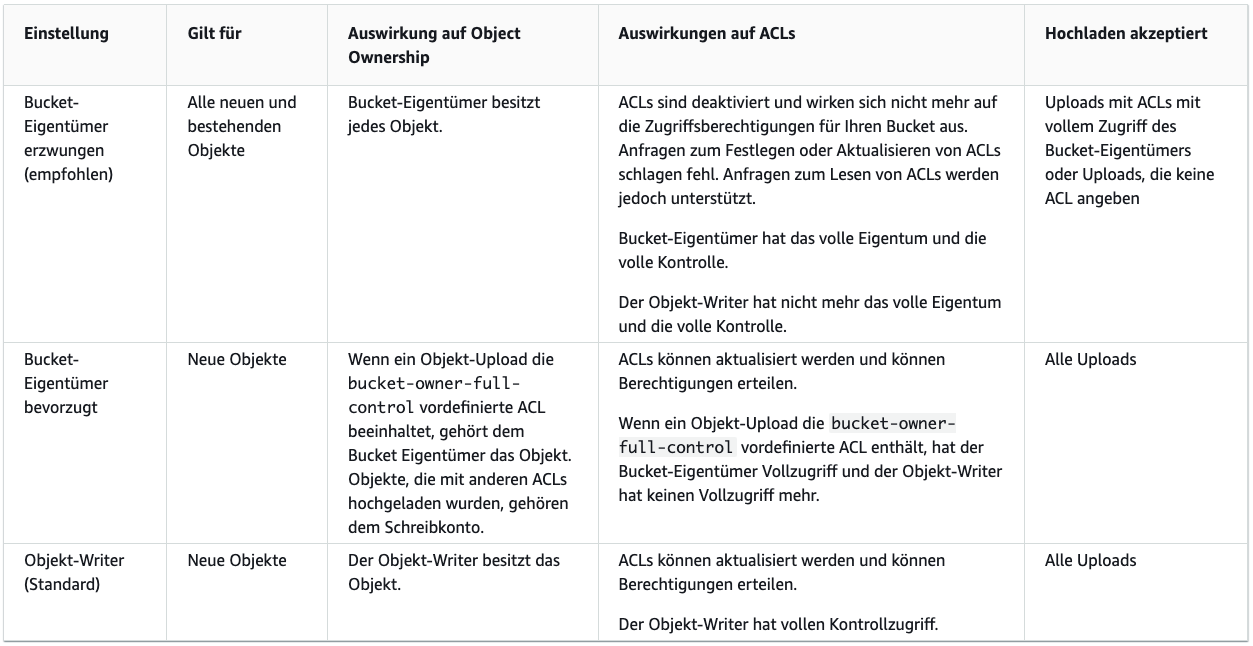
\includegraphics[width=16cm,keepaspectratio]{Pictures/objectOwnershipTable.png}
	\caption{Einstellungen für Object Ownership, \citeurl{aws-iam-s3}}
\end{figure}

Laut \citeauthor{aws-iam-s3} zeigt die obige Tabelle die Auswirkungen, die jede Einstellung für Object Ownership auf ACLs, Objekte, Objekteigentümer und Objekt-Uploads hat.\\

Logging ist ein weiterer Aspekt der Amazon S3-Sicherheit. S3 bietet verschiedene Logging-Optionen, darunter Bucket Logging und Object-Level Logging, die es Benutzern ermöglichen, Zugriffe auf S3-Objekte aufzuzeichnen und zu überwachen. Diese Funktionen sind entscheidend, um Compliance-Anforderungen zu erfüllen und verdächtige Aktivitäten zu erkennen. AWS bietet eine Vielzahl von tools zur Überwachung der Amazon S3 Ressourcen. Darunter die Amazon CloudWatch Alarms, AWS CloudTrail Logs, Amazon S3 Access Logs und die AWS Trusted Advisor.\\

%TODO compliance

\newpage

\textbf{Google Cloud Storage}\\

Auch Google Cloud bietet eine Vielzahl an Sicherheitsfunktionen, um sicherzustellen, dass Daten in der Cloud sicher gespeichert und geschützt sind. Unter anderem die Datenverschlüsselung. Google Cloud bietet genau wie Amazon S3 Serverseitige Verschlüsselung an. Hier unterscheidet man zwischen Google-managed Keys, Customer-managed encryption keys und die Customer-supplied encryption keys. Google-managed encryption ist die Standard Verschlüsselungsoption von Google Cloud. Cloud Storage verschlüsselt die Daten serverseitig, bevor die Daten auf die Festplatte geschrieben werden. 

\begin{quote}
	Die Standard Variante verwaltet für den Nutzer die Encryption Keys in ihrem eigenen Key Management System. Auch Google verwendet für die Verschlüsselung die AES-256 wie AWS. Als Nutzer muss man bei dieser Varianet keine Einstellungen berücksichtigen. Daten werden automatisch verschlüsselt beim Abruf, vgl. \cite{gcp-encrypt}.
\end{quote}

Wenn man mehr Kontrolle über die Schlüssel haben möchte, dann gibt es die Customer-managed encryption Option. Die Schlüssel werden von Cloud KMS (Cloud Key Management Service) erstellt und verwaltet. Diese Schlüssel werden vom Nutzer anschließend extern oder in einem HSM Cluster gespeichert. Customer Keys kann man für indivduelle Objekte benutzen oder einen Bucket so einstellen, dass er einen Standard Key für alle neuen Objekte verwendet. Der erstellte Schlüssel wird für die Verschlüsselung der Objektdaten, die CRC32C Checksum des Objekts und für die MD5 Hash verwendet. Als zusätzlichen Schutz gibt es die Service Agents, auch genannt als service accounts. Diesem Agent kann man bestimmte Rechte geben, sodass es Zugriff auf den gewünschten Encryption Key hat, um damit Objekte verschlüsseln zu können.\\

Zuletzt gibt es noch die Customer-supplied encryption keys. Als zusätzliche Sicherheitsebene zu Google-managed encryption keys können Nutzer ihren eigenen AES-256 Encryption Key bereitstellen, welches als Base64 encoded ist. Bei dieser Variante wird der Schlüssel nicht von Google Cloud gespeichert oder verwaltet. Die Nutzer müssen diese Schlüssel selber verwalten und speichern. Um zukünftige Requests zu validieren speichert Google Cloud einen kryptografischen Hash vom Schlüssel. Jedoch kann der Encryption Key nicht aus dem Hash regeneriert werden oder den Hash nicht zum Entschlüsseln anwenden.\\

Des weiteren gibt es auch in Google Cloud Zugriffskontrolleinstellungen, mit der Nutzer genau steuern können, wer auf ihre Daten zugreifen kann. Den Zugriff kann man auf Bucket- und Objektebene steuern und Benutzern und Gruppen bestimmte Rollen zuweisen. Dabei wird zwischen Uniform und Fine-grained unterschieden. Uniform Access Control (UAC) ermöglicht es, den Zugriff auf einen gesamten Bucket in Google Cloud Storage auf der Ebene von Rollen zuzuweisen. Dazu können verschiedene vordefinierte Rollen wie "Leser", "Schreiber" oder "Besitzer" verwendet werden, die festlegen, welche Aktionen ein Benutzer auf dem Bucket ausführen darf. UAC ist eine einfachere Methode zur Zugriffskontrolle, da die Zugriffsrechte auf Bucket-Ebene vergeben werden. Das bedeutet, dass alle Objekte in dem Bucket automatisch dieselben Zugriffsrechte haben.\\

Fine-Grained Access Control (FGAC) hingegen ermöglicht es, die Zugriffskontrolle auf die Ebene von Objekten oder sogar auf Teile von Objekten herunterzubrechen. Das bedeutet, dass jeder Benutzer oder jede Gruppe individuelle Zugriffsrechte auf bestimmte Objekte oder Teile von Objekten haben kann. Mit FGAC kann man sehr granulare Zugriffssteuerungen implementieren. Es ist eine mächtige Methode, aber auch komplexer und zeitaufwändiger zu implementieren als UAC. Mit Cloud IAM können auch rollenbasierte Zugriffssteuerungen für Bucket- unObjektebene ähnlich wie bei AWS umgesetzt werden.\\

Weitere Funktionen die Google Cloud anbietet ist Objekt Versioning, Audit Logging, Bucket Locks, VPC Service Controls, Data Loss Prevention und Identity-Aware Proxy.


\subsubsection{Hochverfügbarkeit}

\textbf{Amazon S3}\\

Amazon S3 ist ein skalierbarer und hochverfügbarer Objekt Storage, der eine Verfügbarkeit von 99.99 Prozent garantiert.\glqq Designed to provide 99.999999999 percent durability and 99.99 percent availability of objects over a given year.\grqq, \cite{aws-availability}\\

Dies wird durch die Verwendung von Multi-Availability Zone Architekturen erreicht, die eine automatische Replikation von Daten in verschiedenen physischen Standorten ermöglichen. Die Multi-Availability Zone Architektur von Amazon S3 basiert auf der Aufteilung von Daten in mehrere geografisch getrennte Verfügbarkeitszonen (AZs). Jede AZ besteht aus mehreren physischen Rechenzentren, die sich in einem geografisch getrennten Gebiet befinden. Jede AZ ist vollständig unabhängig und bietet eine hohe Redundanz und Verfügbarkeit. Wenn ein Benutzer ein Objekt in Amazon S3 hochlädt, wird es automatisch in mehrere AZs repliziert.um sicherzustellen, dass das Objekt auch bei AUsfällen in einer AZ weiterhin verfügbar ist. Im Falle eines Ausfalls einer AZ wird Amazon S3 automatisch die Anfragen auf eine andere AZ umleiten, um eine ununterbrochene Verfügbarkeit des Objekts sicherzustellen. Durch die Cross-Region Replikation werden Daten automatisch in andere AWS-Regionen repliziert. Dadurch kann eine hohe Verfügbarkeit der Daten im Falle eines Ausfalls einer gesamten AWS-Region gewährleistet werden.\\

Amazon S3 bietet auch eine hohe Verfügbarkeit von Metadaten, die für den Zugriff auf Objekte verwendet werden. Metadaten werden automatisch in mehrere AZs repliziert, um sicherzustellen, dass die Metadaten auch im Falle eines Ausfalls einer AZ verfügbar bleiben. Zusätzlich zu Multi-Availability Zone Architekturen verwendet Amazon S3 auch Fehlerkorrektur- und Erkennungsmechanismen wie CRC-Prüfungen, um die Integrität von Daten sicherzustellen und sicherzustellen, dass die gespeicherten Daten stets korrekt sind.\\

Durch Aktivierung der Versionierung wird jeder Objektversion, die in einem Amazon S-Bucket gespeichert ist, eine eindeutige Versions-ID zugewiesen. Wenn eine Objektversion versehentlich gelöscht oder überschrieben wird, kann die vorherige Version wiederhergestellt werden.\\

Um eine hohe Verfügbarkeit bereitzustellen, stell Amazon S3 außerdem noch die S3-Transfer Acceleration zur Verfügung. Durch die Verwendung von Amazon S3-Transfer Acceleration können Benutzer die Übertragung großer Datenmengen beschleunigen, indem ein optimierter Netzwerkpfad genutzt wird. Dadurch kann de Verfügbarkeit der Daten verbessert werden, indem Verbindungsprobleme minimiert werden.\\

Um die Leistung von Amazon S3 zu überwachen und auf mögliche Probleme reagieren zu können wird CloudWatch bereitgestellt. Dadurch können Ausfallzeiten minimiert werden und herausfinden, an welchen Momenten die Verfügbarkeit am geringsten ist.

Insgesamt bietet Amazon S3 eine hochverfügbare und zuverlässige Speicherlösung, die durch Multi-Availability Zone Architekturen und Fehlerkorrekturmechanismen eine Verfügbarkeit von 99,99 Prozent gewährleistet.\\

\textbf{Google Cloud Storage}\\

Auch Google Cloud Storage bietet die Multi-Region Storage an. Dies ermöglicht die Speicherung von Daten in mehreren Regionen weltweit. Dadurch werden die Daten redundant repliziert und bleiben auch im Falle eines Ausfalls einer Region verfügbar.\\ 

Object Versioning bietet wie AWS die Möglichkeit Objektversionen beizubehalten. Dadurch können vorherige Versionen von Objekten wiederhergestellt werden, falls sie versehentlich gelöscht oder überschrieben werden.\\

Mit der Bucket- und Objekt Replikation können Daten automatisch in andere Regionen oder Projekte repliziert werden. Dies ermöglicht eine geografische Redundanz und verbessert die Verfügbarkeit der Daten.\\

Google Cloud Storage verwendet verteilte Speichersysteme eine redundante Infrastruktur, um eine hohe Datensicherheit- und Verfügbarkeit zu gewährleisten. Die Daten werden in mehreren Datenzentren repliziert, um Ausfälle zu vermeiden.\\

Ein weiterer Punkt ist die Monitoring und Fehlererkennung wie Stackdriver Monitoring, um die Leistung und Verfügbarkeit von google Cloud Storage zu überwachen und auf potenzielle Probleme zu reagieren.

\newpage

\subsubsection{Kosten}

In diesem Abschnitt werden die Kosten von Amazon S3 und Google Cloud Storage betrachtet. Dabei werden die allgemeinen Kosten erläutert für welche die Cloud Provider Gebühren fordern. Bei der Kostenanalyse werden anschließend die Daten von leoticket genommen und eine grobe Abschätzung der Kosten durchgeführt.\\

Amazon S3 setzt Gebühren für die Speicherung, Anforderungen und Datenabrufe, Datenübertragung, Verwaltung und Analyse, Replikation und S3 Objekt Lambda. Für die Speicherung ist die Gebühr abhängig von der Größe der Objekte, der Speicherdauer während des Monats und der Speicherklasse. Es gibt verschiedene Speicherklassen zur Auswahl, die für verschiedenen Use Cases geeignet sind. Das wären die S3 Standard, S3 Intelligent-Tiering, S3 Standard – Infrequent Access, S3 One Zone – Infrequent Access, S3 Glacier Instant Retrieval, S3 Glacier Flexible Retrieval (früher S3 Glacier) und S3 Glacier Deep Archive. S3 Glacier wird in dieser Arbeit nicht behandelt, da leoticket keine Anwendung für diese Speicherklasse hat. Es werden die Speicherklassen S3 Standard, S3 Intelligent-Tiering, S3 Standard - Infrequent Access und S3 One Zone - Infrequent Access untersucht.

Um das Ganze zu veranschaulichen, werden die Preise durch die untere Tabelle präsentiert.

\begin{figure}[h]
	\centering
	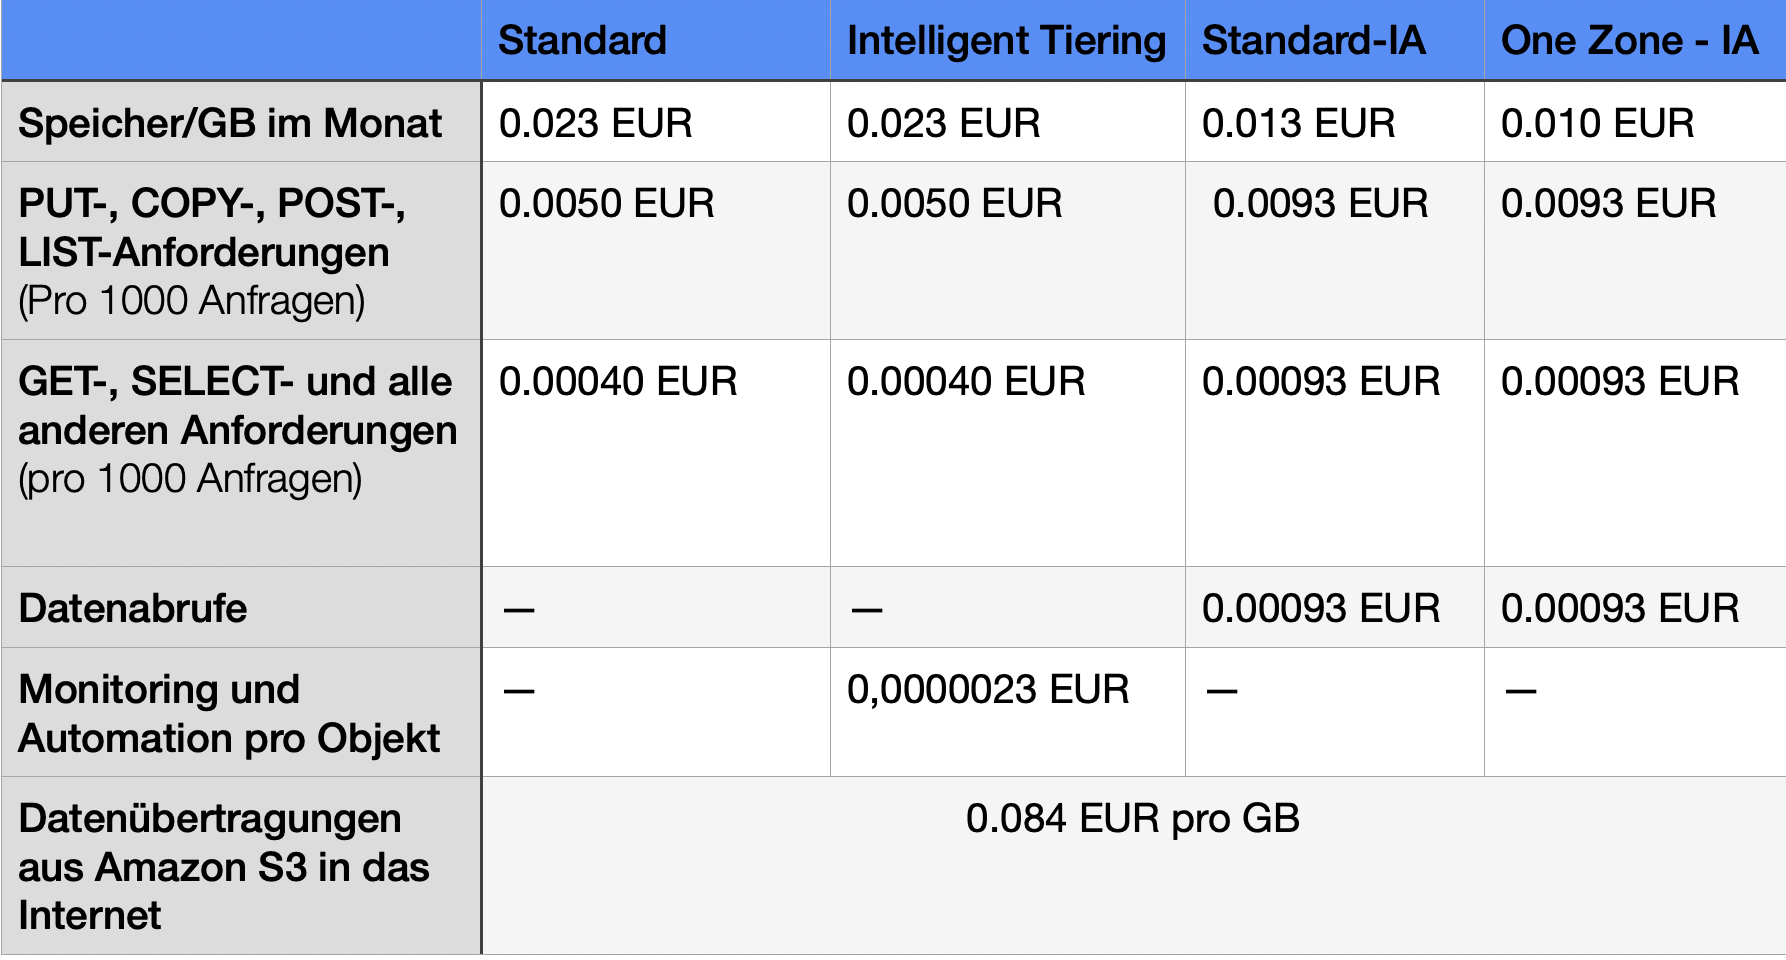
\includegraphics[width=15cm,keepaspectratio]{Pictures/AllgKostenAWS.png}
	\caption{Übersicht der Kosten der AWS S3 Speicherklassen}
\end{figure}

In der obigen Tabelle werden die Standard Preise von den verschiedenen Speicherklassen von Amazon S3 dargestellt. Die One Zone -IA hat dabei die niedrigsten kosten im Vergleich zur Standard Speicherklasse. Jedoch sind die Kosten für die Anfragen beim One zone - IA genauso wie beim Standard - IA höher als beim Standard und Intelligent Tiering. Zusätzlich werden bei Datenabrufen in den Fällen von Standard-IA und One Zone-IA Gebühren von 0.01 USD pro GB erhoben. So sind die Speicherklassen Standard und Intelligent Tiering für häufig abgerufene Daten, bei denen eine sofortige Verfügbarkeit und eine niedrige Latenzzeit erforderlich ist geeignet. Standard bietet eine hohe Leistung und ist ideal für Anwendungen, bei denen schneller Zugriff auf die Daten erforderlich ist. Die Intelligent Tiering eignet sich für Daten mit wechselndem Zugriffsverhalten. Sie analysiert das Zugriffsmuster der Objekte und verschiebt sie automatisch zwischen zwei Zugriffstiers. Dadurch kann man Kosten sparen, da man für den tatsächlichen Zugriff auf die Daten bezahlt und nicht für eine dauerhafte Speicherung in der teureren Speicherklassen.\\

Standard-IA und One Zone-IA bieten kostengünstigere Optionen für die Speicherung der Daten. Die Standard-IA ist für Daten geeignet, auf die weniger häufig zugegriffen wird, aber bei Bedarf schnell verfügbar sein müssen. Im Vergleich zur Standardklasse sind die Kosten für die Speicherung niedriger, aber es fallen zusätzliche Gebühren für den Datenabruf an. Wenn Daten von zwei Speicherklassen hergeschoben werden, dann fallen Kosten für den Speicherklassenwechsel an. Diese hängen von der Datenmenge ab, die verschoben werden.\\

Die One Zone-IA ist für Daten geeignet, auf die selten abgerufen werden, jedoch mit einer Einschränkung. Anders als bei den anderen Speicherklassen wird One Zone-IA nur in einem einzelnen Availability Zone in einer bestimmten Region gespeichert. Dies bedeutet, dass die Daten in einer einzigen AZ verfügbar sind und ein potenzieller Datenverlust auftreten kann, wenn diese AZ nicht verfügbar ist.\\

Bei der Replikation von Daten zahlt man gebühren für die Speicherung in den ausgewählten Ziel-S3-Speicherklassen, für die primäre Kopie, für Replikations-PUT Anforderungen und für anwendbare Gebühren für den Speicherabruf mit seltenem Zugriff. Laut aws preise zahlt man auch für den regionenübergreifenden Datentransfer OUT von S3 zu jeder Zielregion. Die Preise für Speicher- und PUT-Anfragen für die replizierte Kopie basieren auf den ausgewählten AWS-Zielregionen, während die Preise für Datenübertragungen zwischen den Regionen auf der AWS-Quellregion basieren. Wenn man S3 Replication Time Control nutzt, zahlt man eine Datenübertragungsgebühr für die Replikationszeitsteuerung sowie die Gebühren für S3-Replikationsmetriken, die zum selben Tarif abgerechnet werden wie angepasste Amazon-CloudWatch-Metriken. Die kosten für die S3 Replication Time Control-Datenübertragung beträgt pro GB 0.015 USD. https://aws.amazon.com/de/s3/pricing/ \\


Auch bei der Objekt Versionierung fallen Kosten an, wenn man ältere Versionen von Objekten beibehalten möchte. Die Kosten beziehen sich auf den zusätzlichen Speicherplatz, der für die Aufbewahrung der Versionen verwendet wird. Für das Tagging von benutzerdefinierten Metadaten bei Objekten selbst fallen keine direkten Kosten an. Allerdings können Kosten für das Abrufen von Tags über die S3-API(z.B. mit der ListObjects- oder GetObject-Operationen) anfallen, da dies als Datenabruf betrachtet wird und entsprechende Gebühren gemäß den AWS-Preisen Datenzugriff erhoben werden. Es ist zu beachten, dass die genauen Preise für Objektversionierung und Tagging von Amazon S3 sich im Laufe der Zeit ändern können.\\

Die genauen Preise und Kostendetails für S3 Standard IA können sich im Laufe der Zeit ändern. Es wird empfohlen, die aktuellsten Informationen auf der offiziellen AWS-Preisseite oder im AWS-Kostenrechner zu überprüfen, um eine genaue Kosteneinschätzung zu erhalten.


\subsubsection{Performance}




\subsubsection{API Anbindung}

\subsection{Bereitstellung der Dateien}

\section{Auswahl des Speichersystems}

In diesem Abschnitt wird durch eine Kosten-, und Performance Analyse die Speichersysteme ausgewertet und eine Auswahl getroffen. Die Kalkulationsergebnisse werden zum Schluss dargestellt.

\subsection{Kostenanalyse}
\subsection{Performance Analyse}
\subsection{Kalkulationsergebnisse}